\documentclass[a4paper, 12pt]{article}

\usepackage{fontspec}
\usepackage{polyglossia}
\defaultfontfeatures{Ligatures=TeX}
\setdefaultlanguage{russian}
\setotherlanguage{english}
\setmainfont{Times New Roman}
\newfontfamily{\latinfont}{Times New Roman}
\newfontfamily{\cyrillicfont}{Times New Roman}
\newfontfamily{\cyrillicfonttt}{Courier New}

\usepackage{geometry}
\usepackage{amsmath}
\usepackage{amssymb}
\usepackage{amsfonts}
\usepackage{graphicx}
\usepackage{float}
\usepackage{wrapfig}
\usepackage{subcaption}
%\usepackage[caption=false]{subfig}
\geometry{right=20mm}
\geometry{left=20mm}
\geometry{top=20mm}
\geometry{bottom=20mm}

\usepackage{indentfirst}
\usepackage[outputdir=auxiliary]{minted}

\graphicspath{{../img/}}
\DeclareMathOperator{\R}{\mathbb{R}}
\DeclareMathOperator{\C}{\mathbb{C}}
\renewcommand{\Re}{\mathrm{Re}}
\renewcommand{\Im}{\mathrm{Im}}


\DeclareMathOperator{\LA}{%
    \begin{bmatrix}
        0& 1& 0\\
        0& 0& 1\\
        0.1& 0.3& 0.2
    \end{bmatrix}}
\DeclareMathOperator{\Lb}{%
    \begin{bmatrix}
        0.1\\
        -0.3\\
        0.2
    \end{bmatrix}}
\DeclareMathOperator{\LC}{%
    \begin{bmatrix}
        0& 0& 1
    \end{bmatrix}}
\DeclareMathOperator{\I}{%
    \begin{bmatrix}
        1& 0& 0\\
        0& 1& 0\\
        0& 0& 1
    \end{bmatrix}}

\usepackage{xifthen}
\newcommand{\yk}[1][]{%
    \ifthenelse{\isempty{#1}}%
    {y_{k}}%
    {y_{k+#1}}%
}
\newcommand{\xk}[1][]{%
    \ifthenelse{\isempty{#1}}%
    {x_{k}}%
    {x_{k+#1}}%
}
\newcommand{\uk}[1][]{%
    \ifthenelse{\isempty{#1}}%
    {u_{k}}%
    {u_{k+#1}}%
}

\begin{document}
    \begin{titlepage}
    \begin{center}
        \textit{МИНИСТЕРСТВО ОБРАЗОВАНИЯ И НАУКИ\\
        РОССИЙСКОЙ ФЕДЕРАЦИИ}
        \vspace{1ex}

        федеральное государственное бюджетное образовательное учреждение\\
        высшего профессионального образования
        \vspace{1ex}

        \textbf{САНКТ-ПЕТЕРБУРГСКИЙ НАЦИОНАЛЬНЫЙ ИССЛЕДОВАТЕЛЬСКИЙ УНИВЕРСИТЕТ ИТМО}
        \vspace{13ex}

        Лабораторная работа №3\\
        <<Динамика нелинейных систем>>\\
        по дисциплине <<Моделирование технических систем>>\\
        \vspace{1em}
        Вариант 3\\
    \end{center}
    \vspace{14em}
    \begin{flushright}
        \noindent
        Выполнили:\\
        студенты гр. R4133c\\
        Борисов М. В.\\
        Симонов П.\\
        Мацуганов А. И.\\
        \vspace{1em}
        Преподаватель:\\
        Семенов Д. М.
    \end{flushright}
    \vfill
    \begin{center}
        \large{Санкт-Петербург}\\
        2021 г.\\
    \end{center}
\end{titlepage}

    \setcounter{page}{2}
    \setlength{\parindent}{0pt}

    \section*{Задание 1}
    Дана каноническая модель дискретной системы в пространстве состояний.
    \begin{equation*}
        \left\{
        \begin{aligned}
            \xk[1] &= A\xk + b\uk\\
            \yk &= C\xk
        \end{aligned}
        \right.
    \end{equation*}
    где $x \in \R^3,\,u\in\R,\,y\in\R$. Начальные данные - нулевые.

    \begin{equation*}
        A = \LA,\,b = \Lb,\,C = \LC
    \end{equation*}

    \begin{enumerate}
        \item Перейти к функциональной модели "вход-выход"
        \item Построить передаточную функцию системы
    \end{enumerate}

    \subsection*{Решение}
    Передаточная функция системы выражается известным соотношением
    \begin{equation}
        \label{eq:W}
        W(\lambda) = C(\lambda I - A)^{-1}b
    \end{equation}

    Подставляя в~\eqref{eq:W} данные задания получаем
    \begin{equation}
        W(\lambda) = \LC \left( \lambda \I - \LA \right)^{-1}\Lb =
        \dfrac{0.2\lambda^2 -0.89\lambda-0.3}{\lambda^3 - 0.2\lambda^2 -0.3\lambda-0.1}
    \end{equation}

    Из полученного выражения легко получить систему по модели "вход-выход", зная что
    \begin{equation*}
        \begin{aligned}
            a(\lambda) \tilde{y} &= b(\lambda)\tilde{u}\\
            W(\lambda) &= \dfrac{b(\lambda)}{a(\lambda)}
        \end{aligned}
    \end{equation*}

    Получаем
    \begin{equation*}
        \yk[3] - 0.2 \yk[2] - 0.3 \yk[1] - 0.1 \yk = 0.2 \uk[2] - 0.89 \uk[1] - 0.3 \uk
    \end{equation*}

    \section*{Задание 2}
    Дана функциональная модель дискретной системы в пространстве "вход-выход". Начальные данные - нулевые.

    \begin{equation}
        \yk[3] + 0.1\yk[2] - 0.2\yk[1] - 0.3\yk = 0.3\uk[2] + 0.01\uk[1] + 0.06\uk
    \end{equation}

    Перейти к канонической модели в пространстве состояний.

    \subsection*{Решение}
    Систему вида \[\yk[3] + a_{1}\yk[2] + a_{2}\yk[1] + a_{3}\yk = b_{1}\uk[2] + b_{2}\uk[1] + b_{3}\uk\]
    легко представить в виде модели в пространстве состояний составив соответствующие матрицы $A$, $B$ и $C$
    следующим образом:

    \begin{equation*}
        \left\{
        \begin{aligned}
            \xk[1] &= A\xk + b\uk\\
            \yk &= C\xk
        \end{aligned}
        \right.
    \end{equation*}

    \begin{equation*}
        A =
        \begin{bmatrix}
            -a_1& 1& 0\\
            -a_2& 0& 1\\
            -a_3& 0& 0
        \end{bmatrix}
        =
        \begin{bmatrix}
            -0.1& 1& 0\\
            0.2& 0& 1\\
            0.3& 0& 0
        \end{bmatrix}
        ,\,B =
        \begin{bmatrix}
            b_1\\
            b_2\\
            b_3
        \end{bmatrix}
        =
        \begin{bmatrix}
            0.3\\
            0.01\\
            0.06
        \end{bmatrix}
        ,\,C =
        \begin{bmatrix}
            1& 0& 0
        \end{bmatrix}
    \end{equation*}

    \section*{Задание 3}
    Дана передаточная функция устойчивой непрерывной системы
    \begin{equation}
        W(s) = \dfrac{s+2}{s^2+4s+5}
    \end{equation}

    \begin{enumerate}
        \item Построить переходную функцию данной системы
        \item Найти передаточную функцию дискретной системы, соответствующей исходной, по методу Эйлера.
        \item Получить оценку на шаг дискретезации, при котором система будет устойчивой.
        \item Построить переходную функцию полученной дискретной системы с разными шагами дискретизации - при котором система устойчива и при котором неустойчива.
        \item Найти передаточную функцию дискретной системы, соответствующей исходной, по методу Тастина.
        \item Построить переходную функцию полученной системы.
    \end{enumerate}

    \subsection*{Решение}
    \subsubsection*{Переходная функция исходной системы}
    \begin{figure}[H]
        \centering
        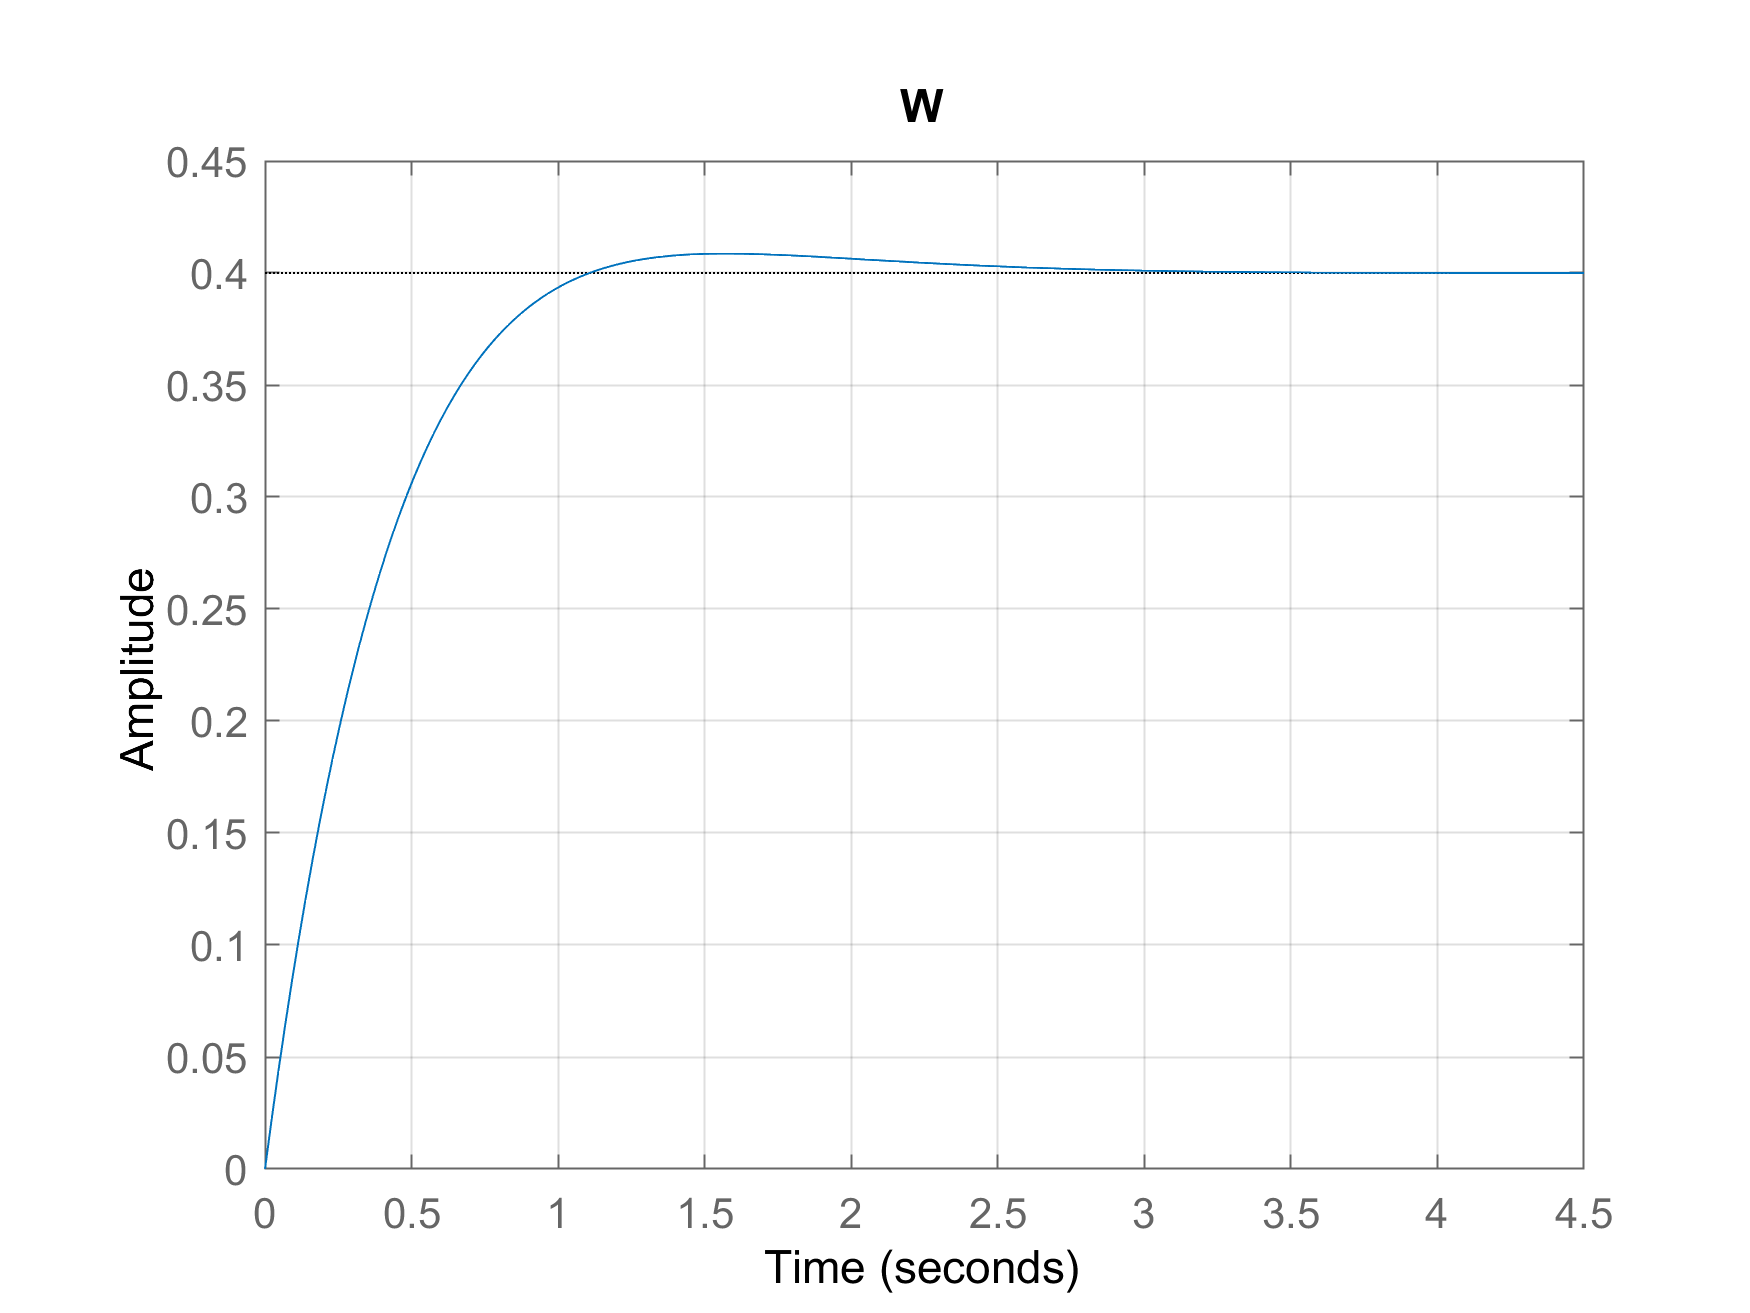
\includegraphics[width=0.5\linewidth]{init.png}
        \caption{Переходной процесс исходной системы}
    \end{figure}

    \subsubsection*{Дискретизация системы}
    \paragraph*{Оценка дискретизации}
    \begin{equation}
        \begin{aligned}
            h &< \min\dfrac{2\left| \Re\,s(A) \right|}{\left| s(A) \right|^2}\\
            h &< 0.8
        \end{aligned}
    \end{equation}

    \paragraph*{Дискретизация по Эйлеру}
    \begin{equation}
        W(z) = \dfrac{hz + 2h^2 - h}{z^2+\left(4\,h-2\right)\,z+5\,h^2-4\,h+1}
    \end{equation}
    \begin{figure}[H]
        \centering
        \begin{subfigure}{0.49\linewidth}
            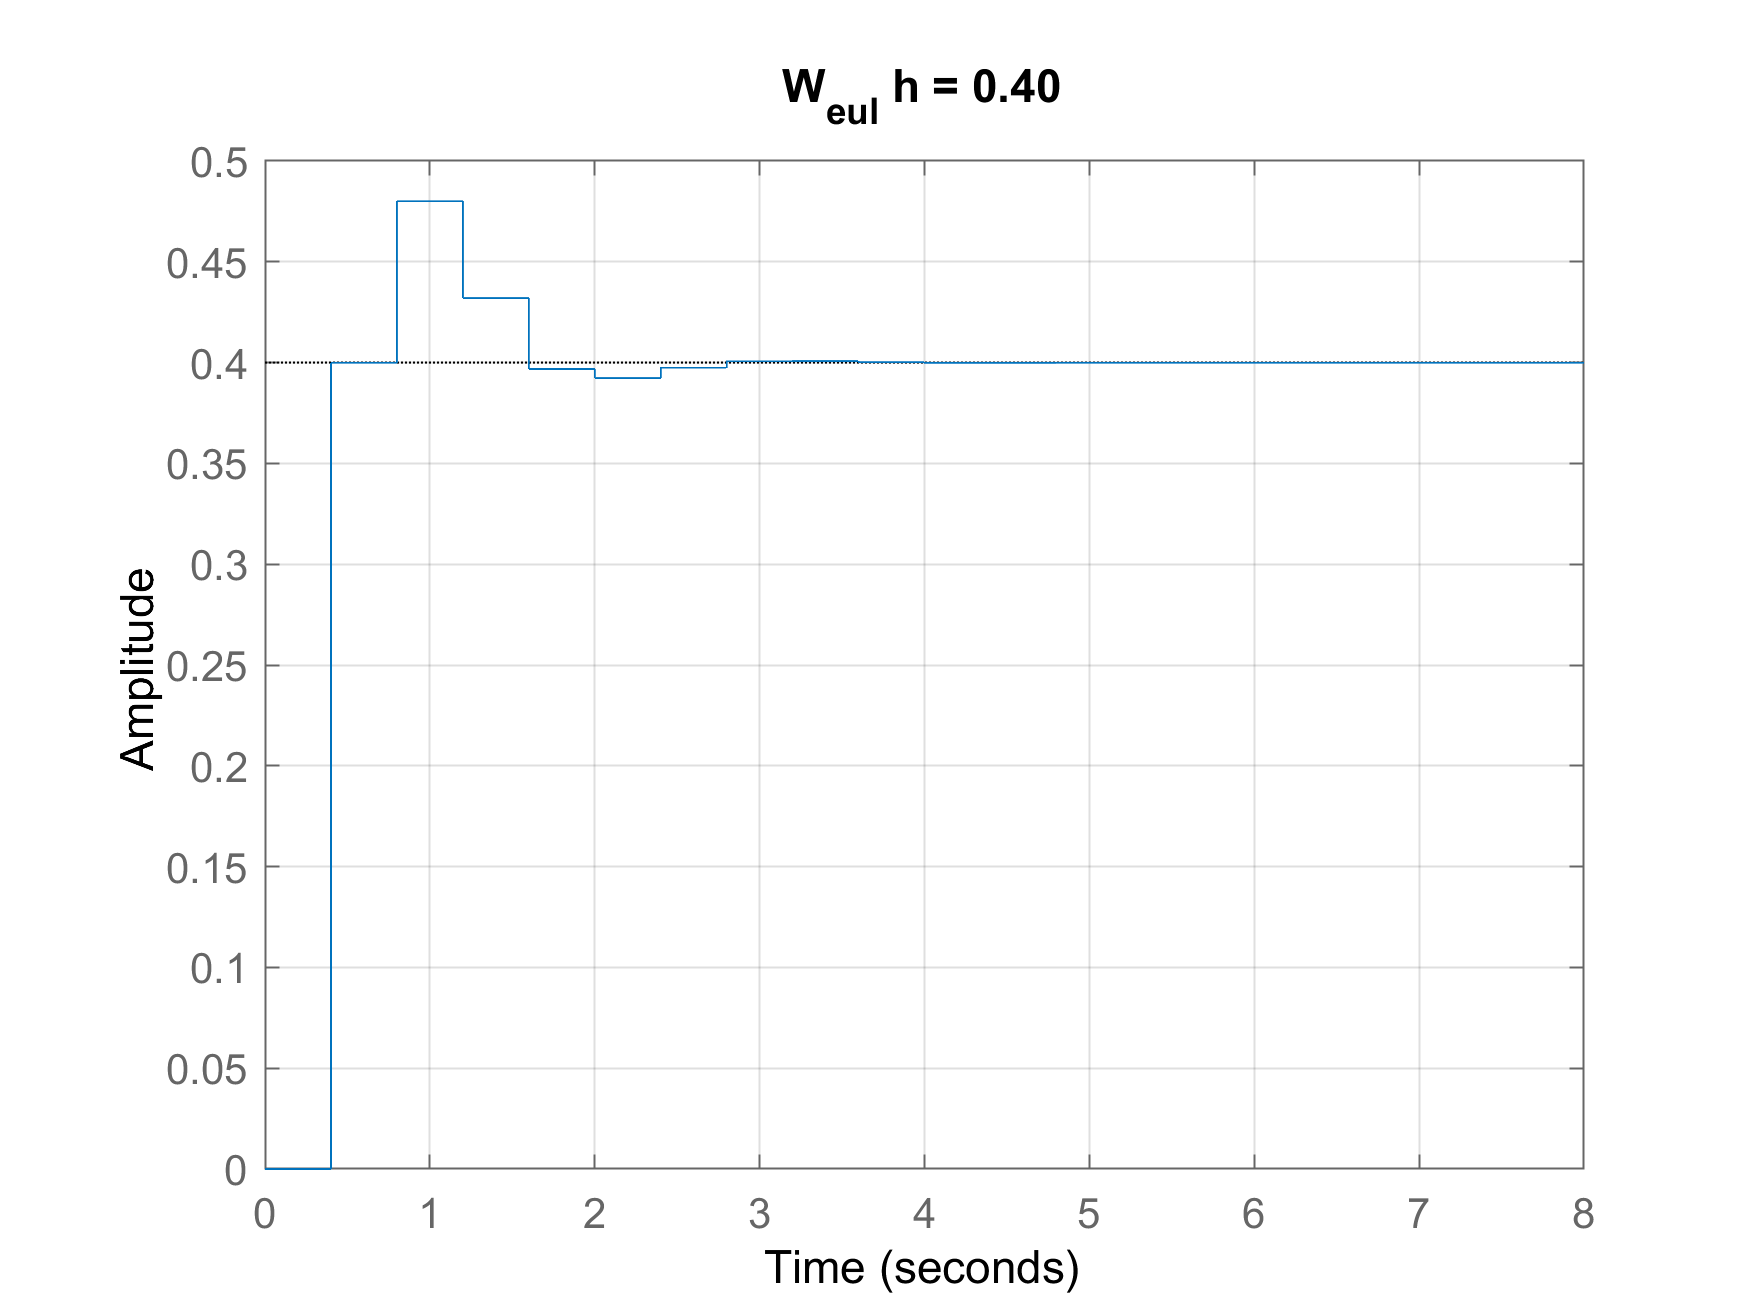
\includegraphics[width=\linewidth]{eulh0.4.png}
        \end{subfigure}
        \begin{subfigure}{0.49\linewidth}
            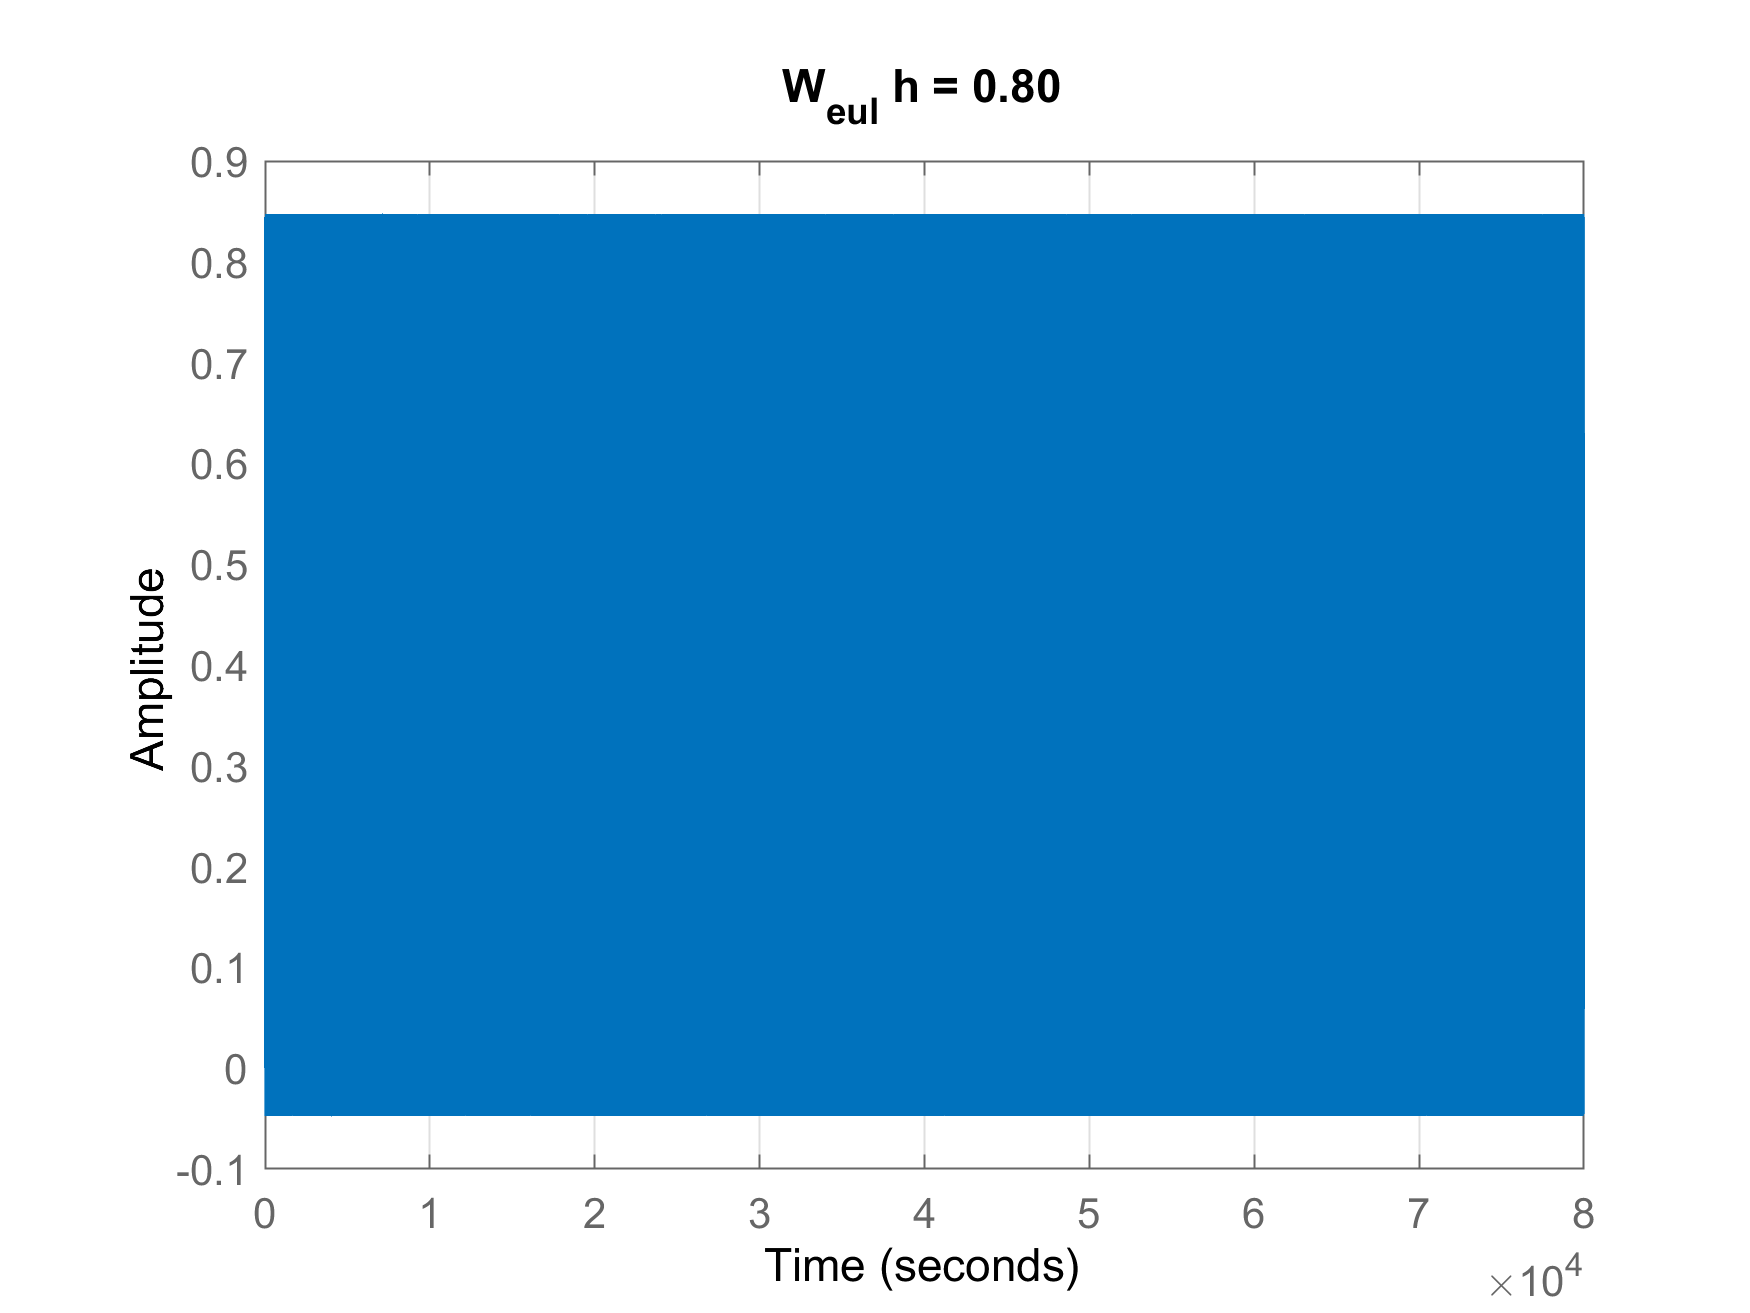
\includegraphics[width=\linewidth]{eulh0.8.png}
        \end{subfigure}
        \begin{subfigure}{0.49\linewidth}
            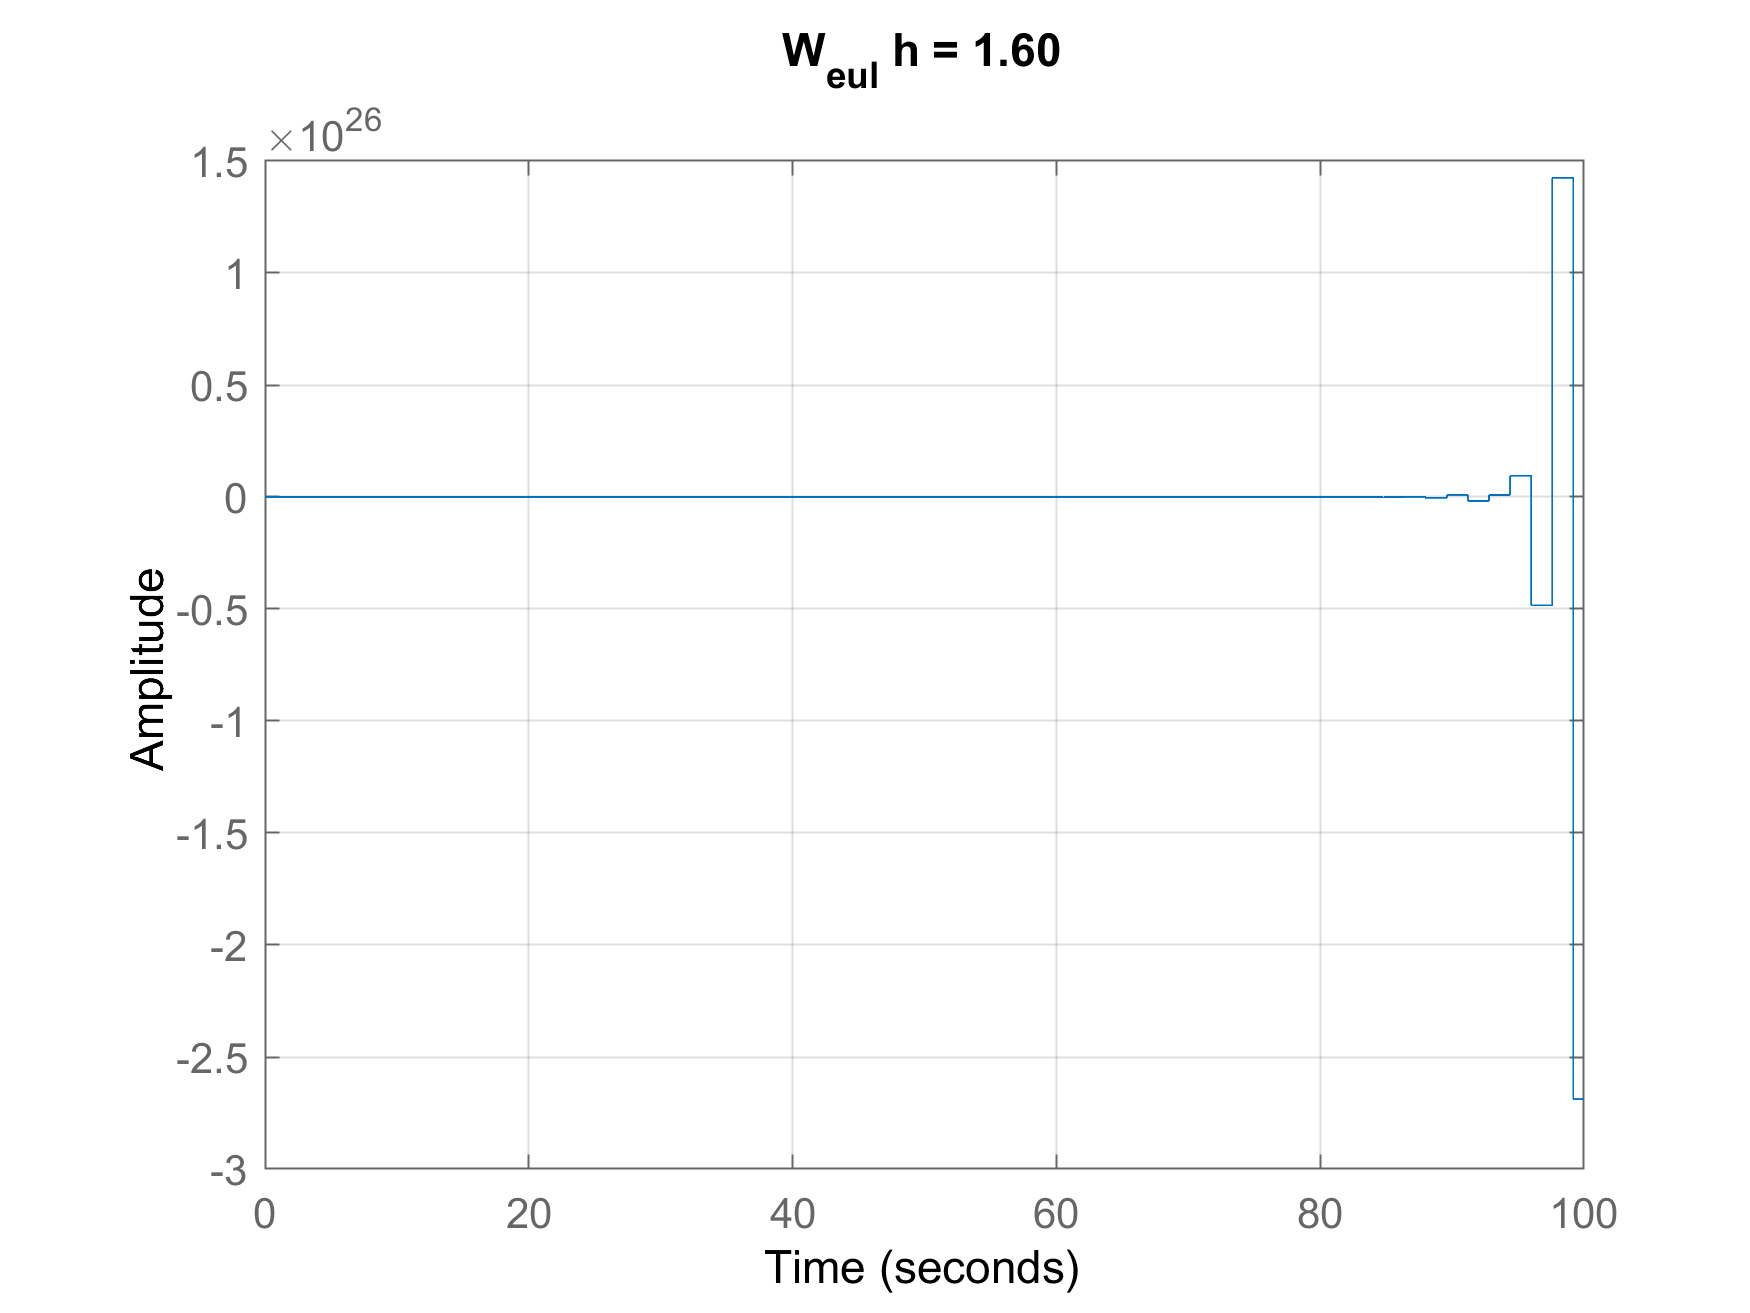
\includegraphics[width=\linewidth]{eulh1.6.png}
        \end{subfigure}
        \begin{subfigure}{0.49\linewidth}
            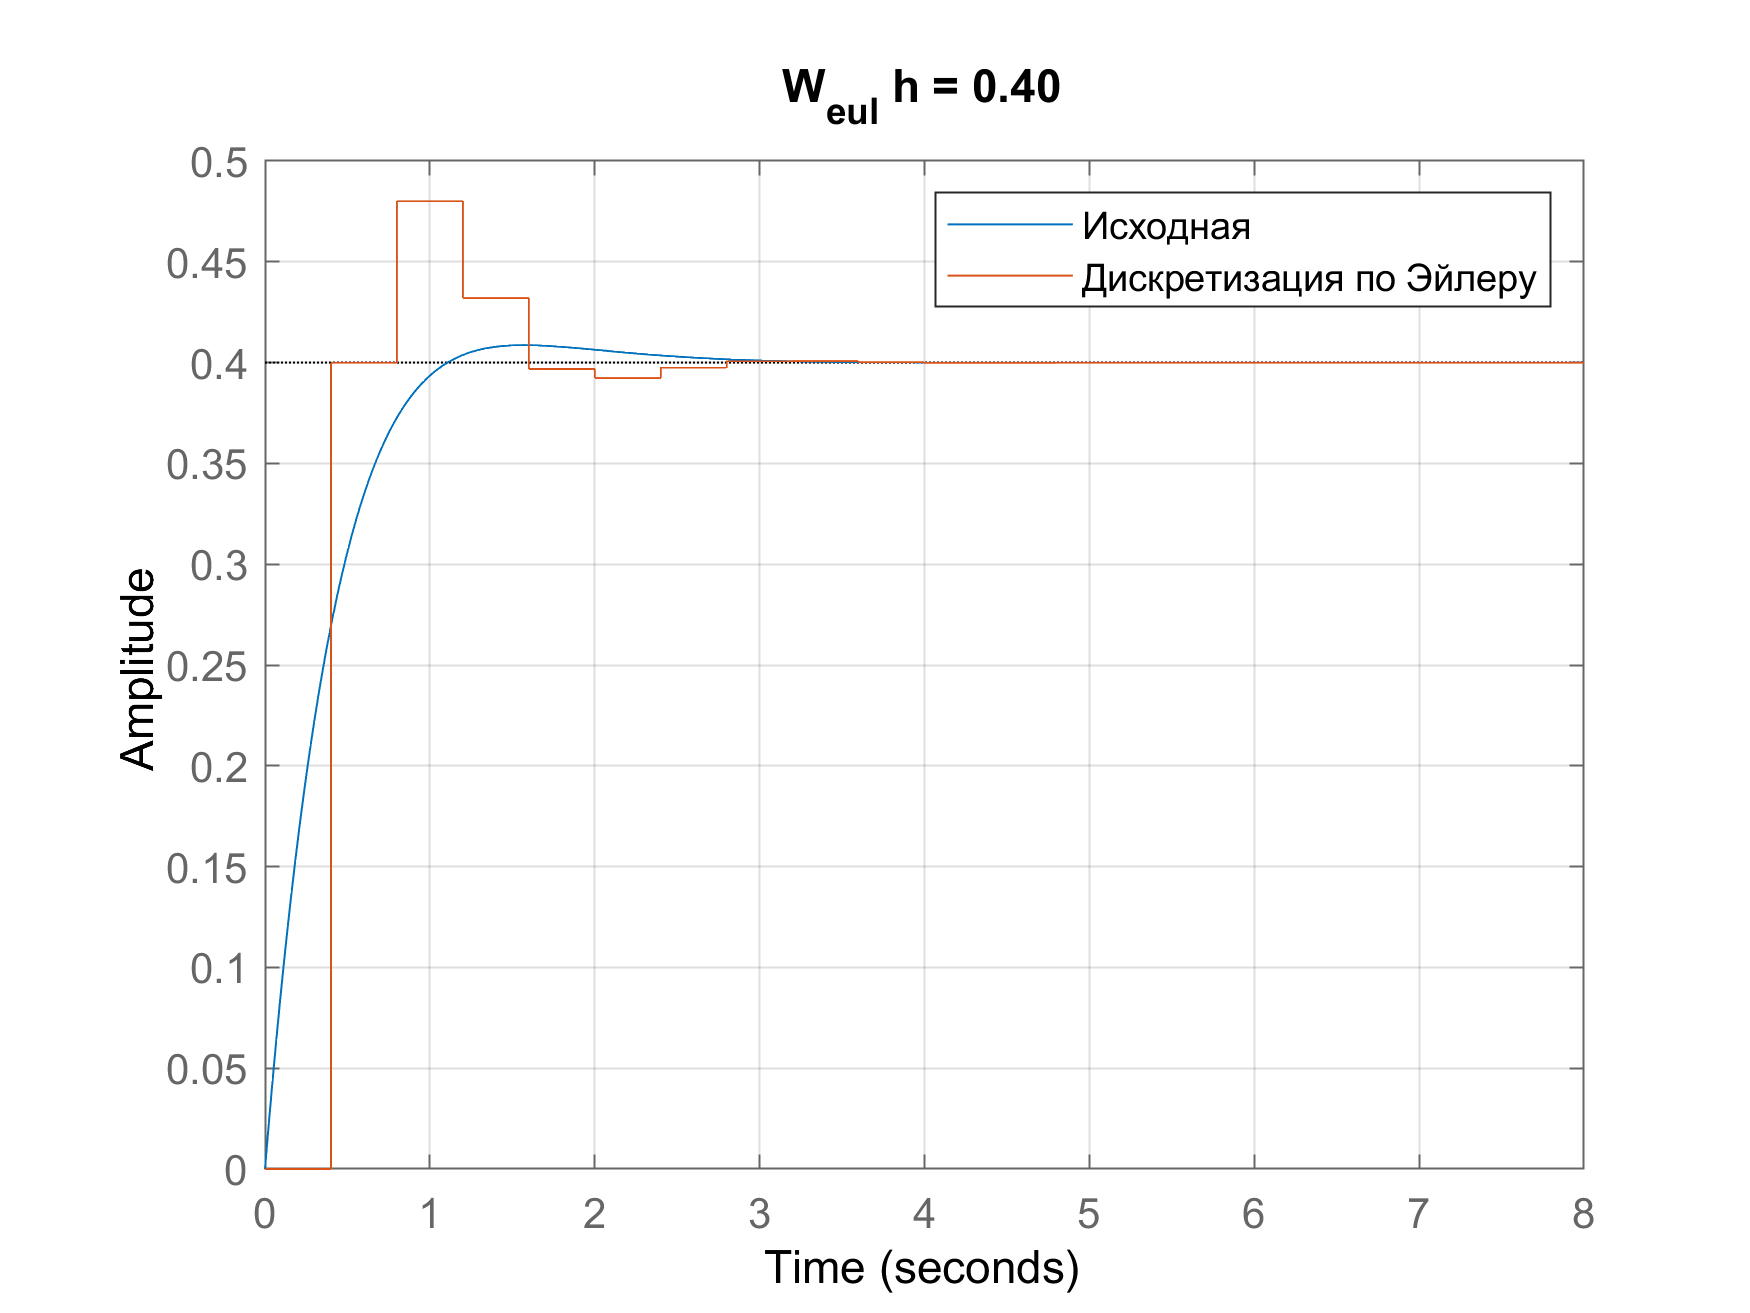
\includegraphics[width=\linewidth]{init-eulh0.4.png}
        \end{subfigure}
        \caption{Переходной процесс системы дискретизированной по Эйлеру}
    \end{figure}

    \paragraph*{Дискретизация по Тастину}
    \begin{equation}
        W(z) = \dfrac{(h+1)z^2 + 2hs + h -1}{\left(5\,h^2+8\,h+4\right)\,z^2+\left(10\,h^2-8\right)\,z+5\,h^2-8\,h+4}
    \end{equation}
    \begin{figure}[H]
        \centering
        \begin{subfigure}{0.49\linewidth}
            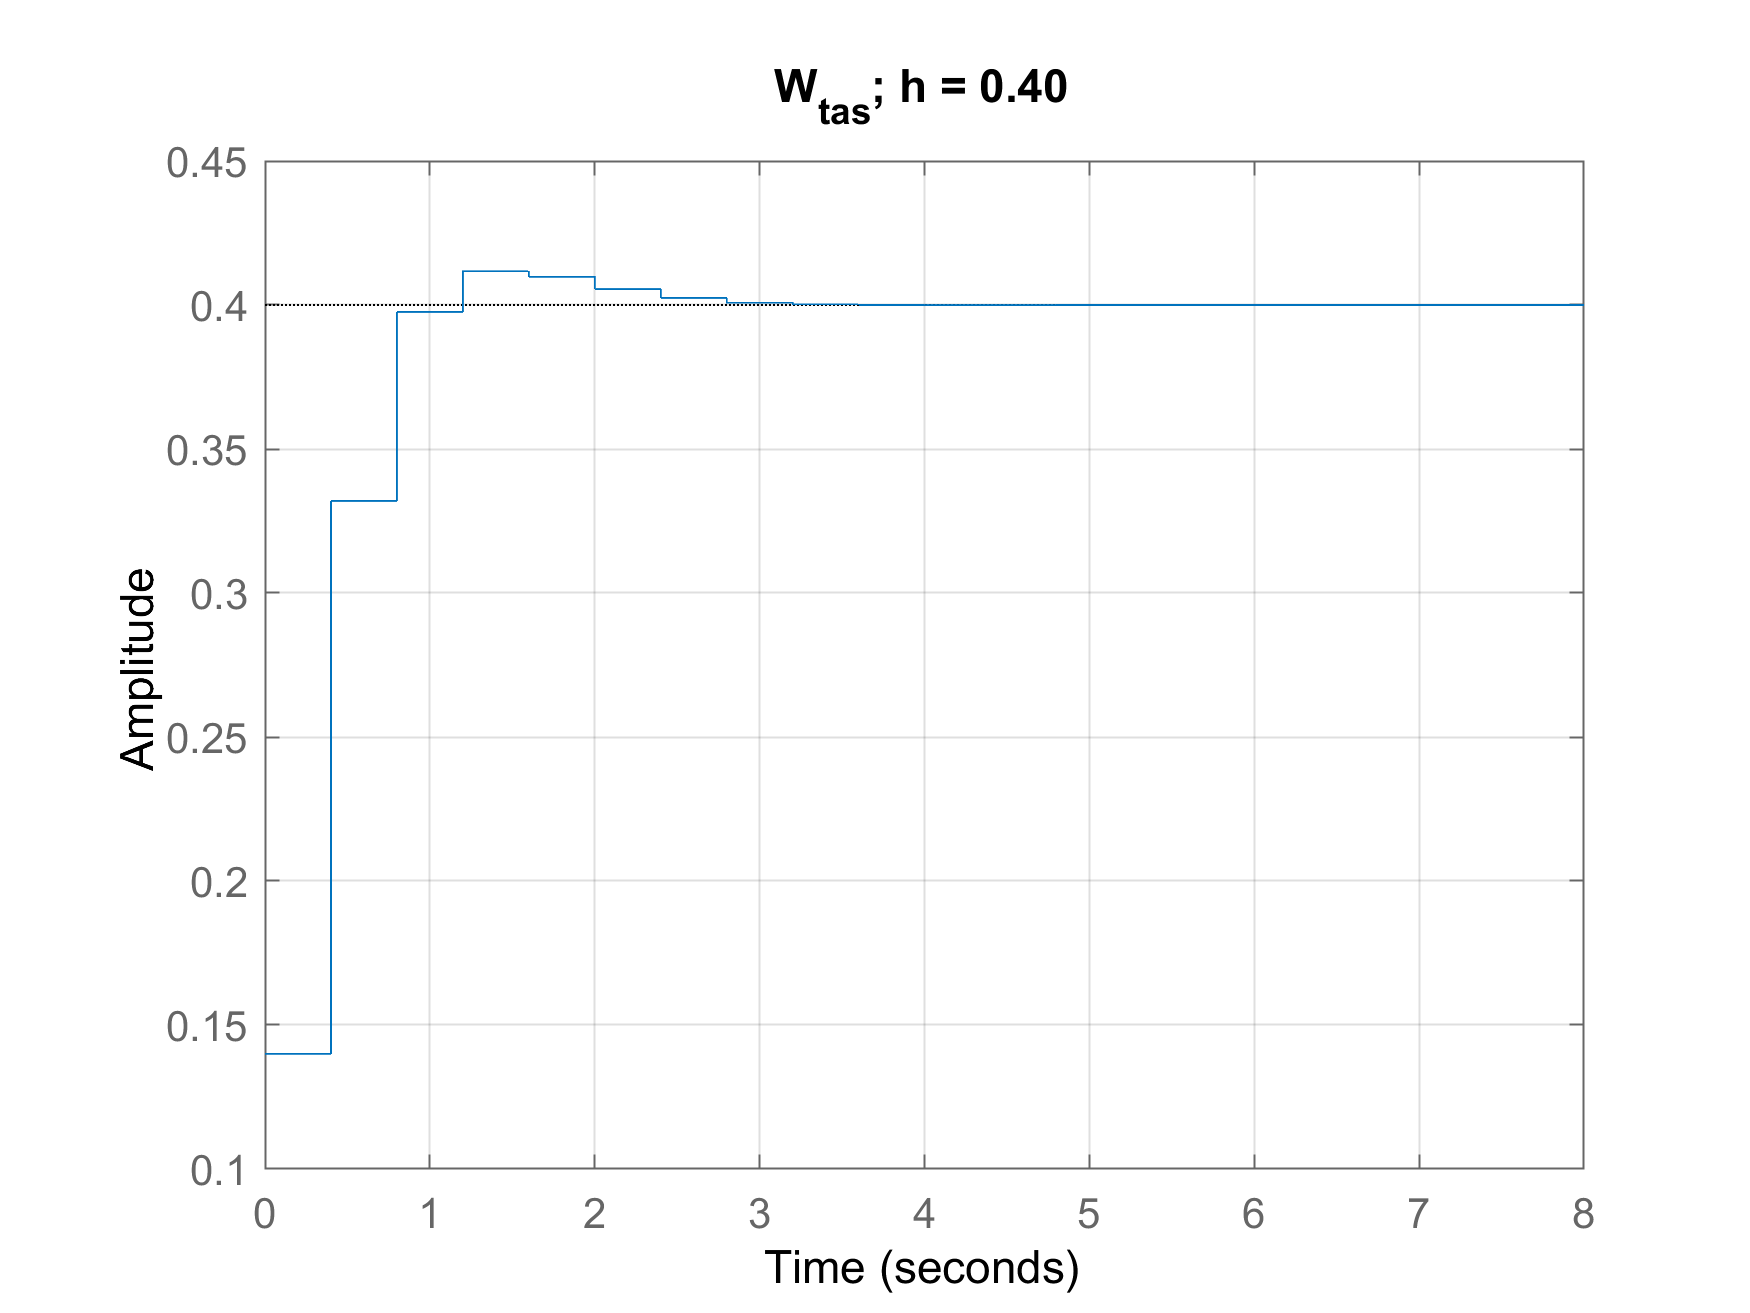
\includegraphics[width=\linewidth]{tash0.4.png}
        \end{subfigure}
        \begin{subfigure}{0.49\linewidth}
            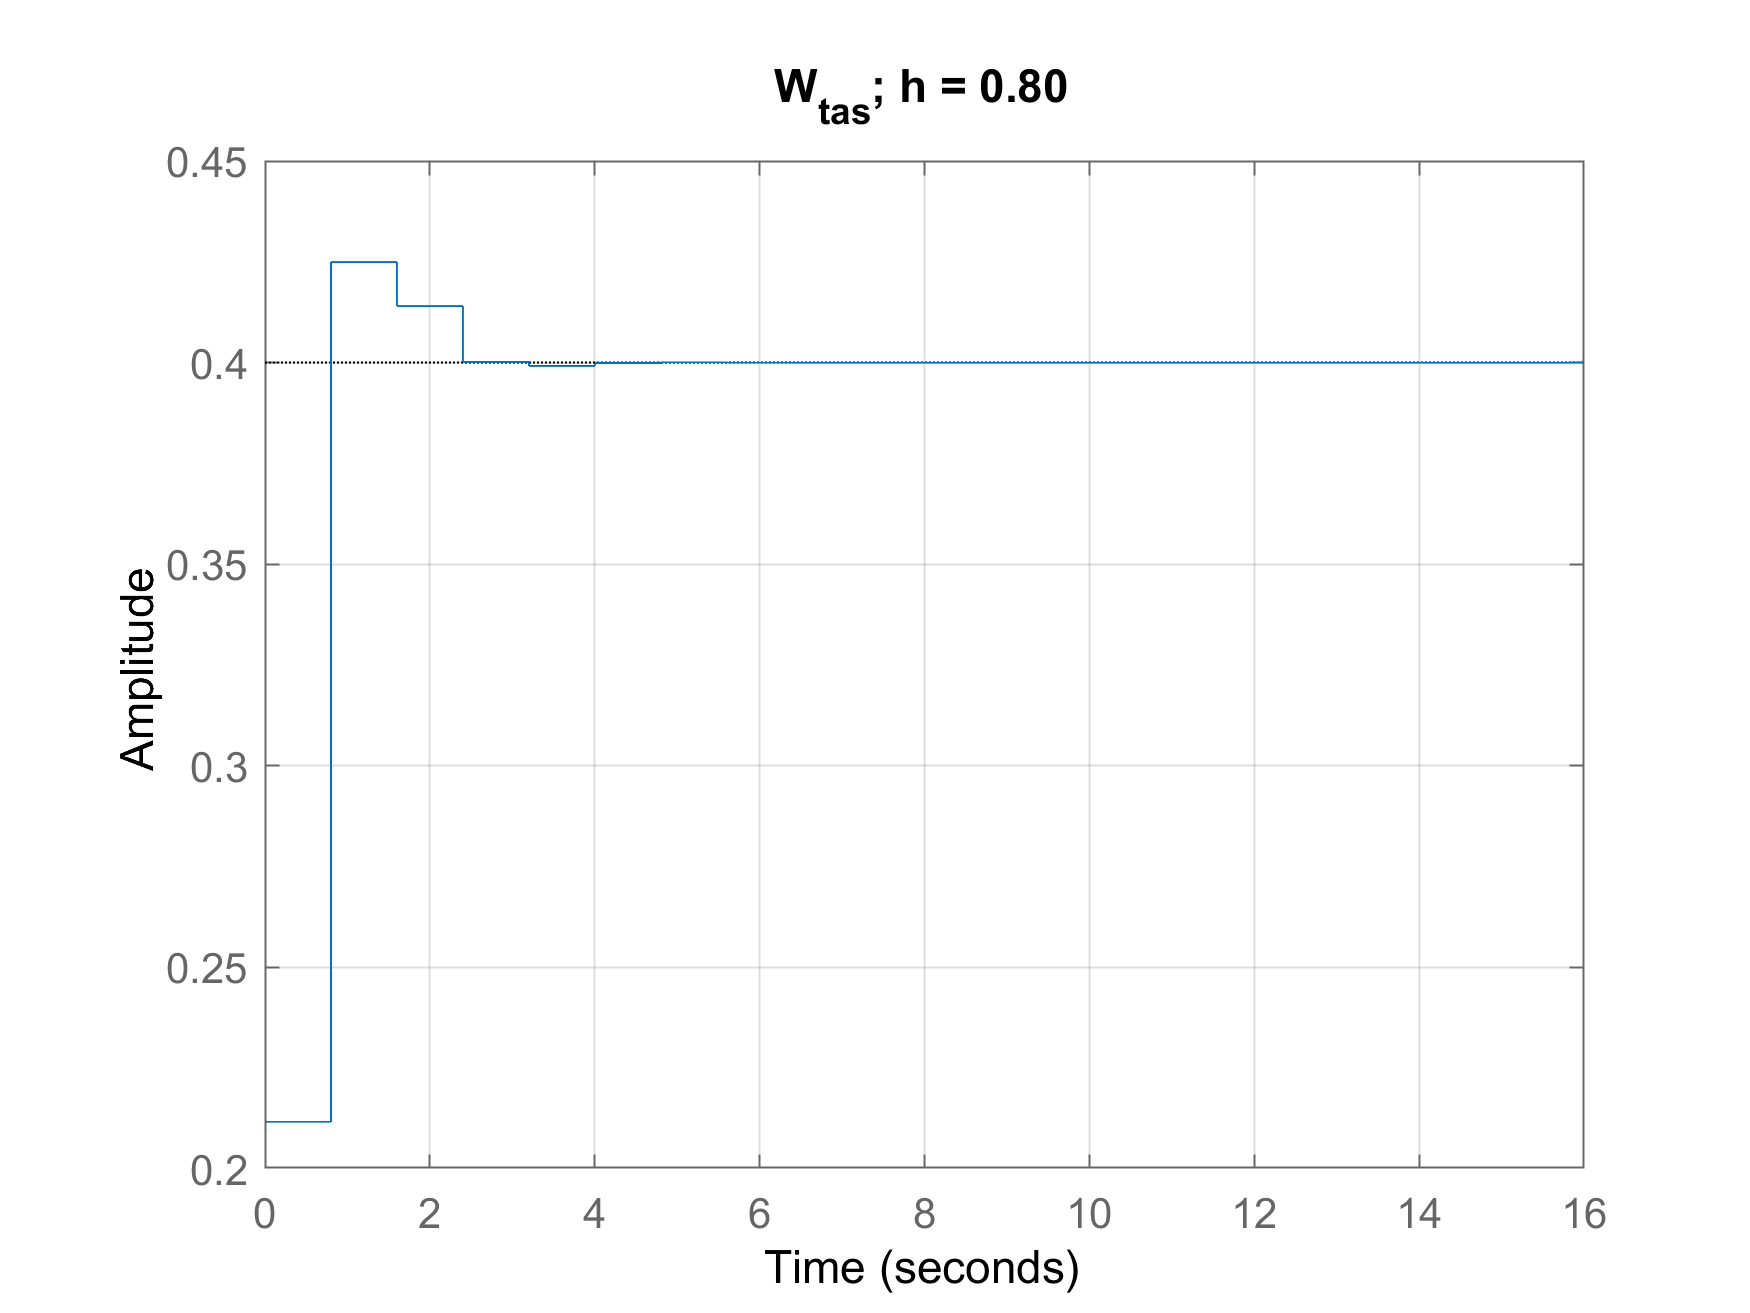
\includegraphics[width=\linewidth]{tash0.8.png}
        \end{subfigure}
        \begin{subfigure}{0.49\linewidth}
            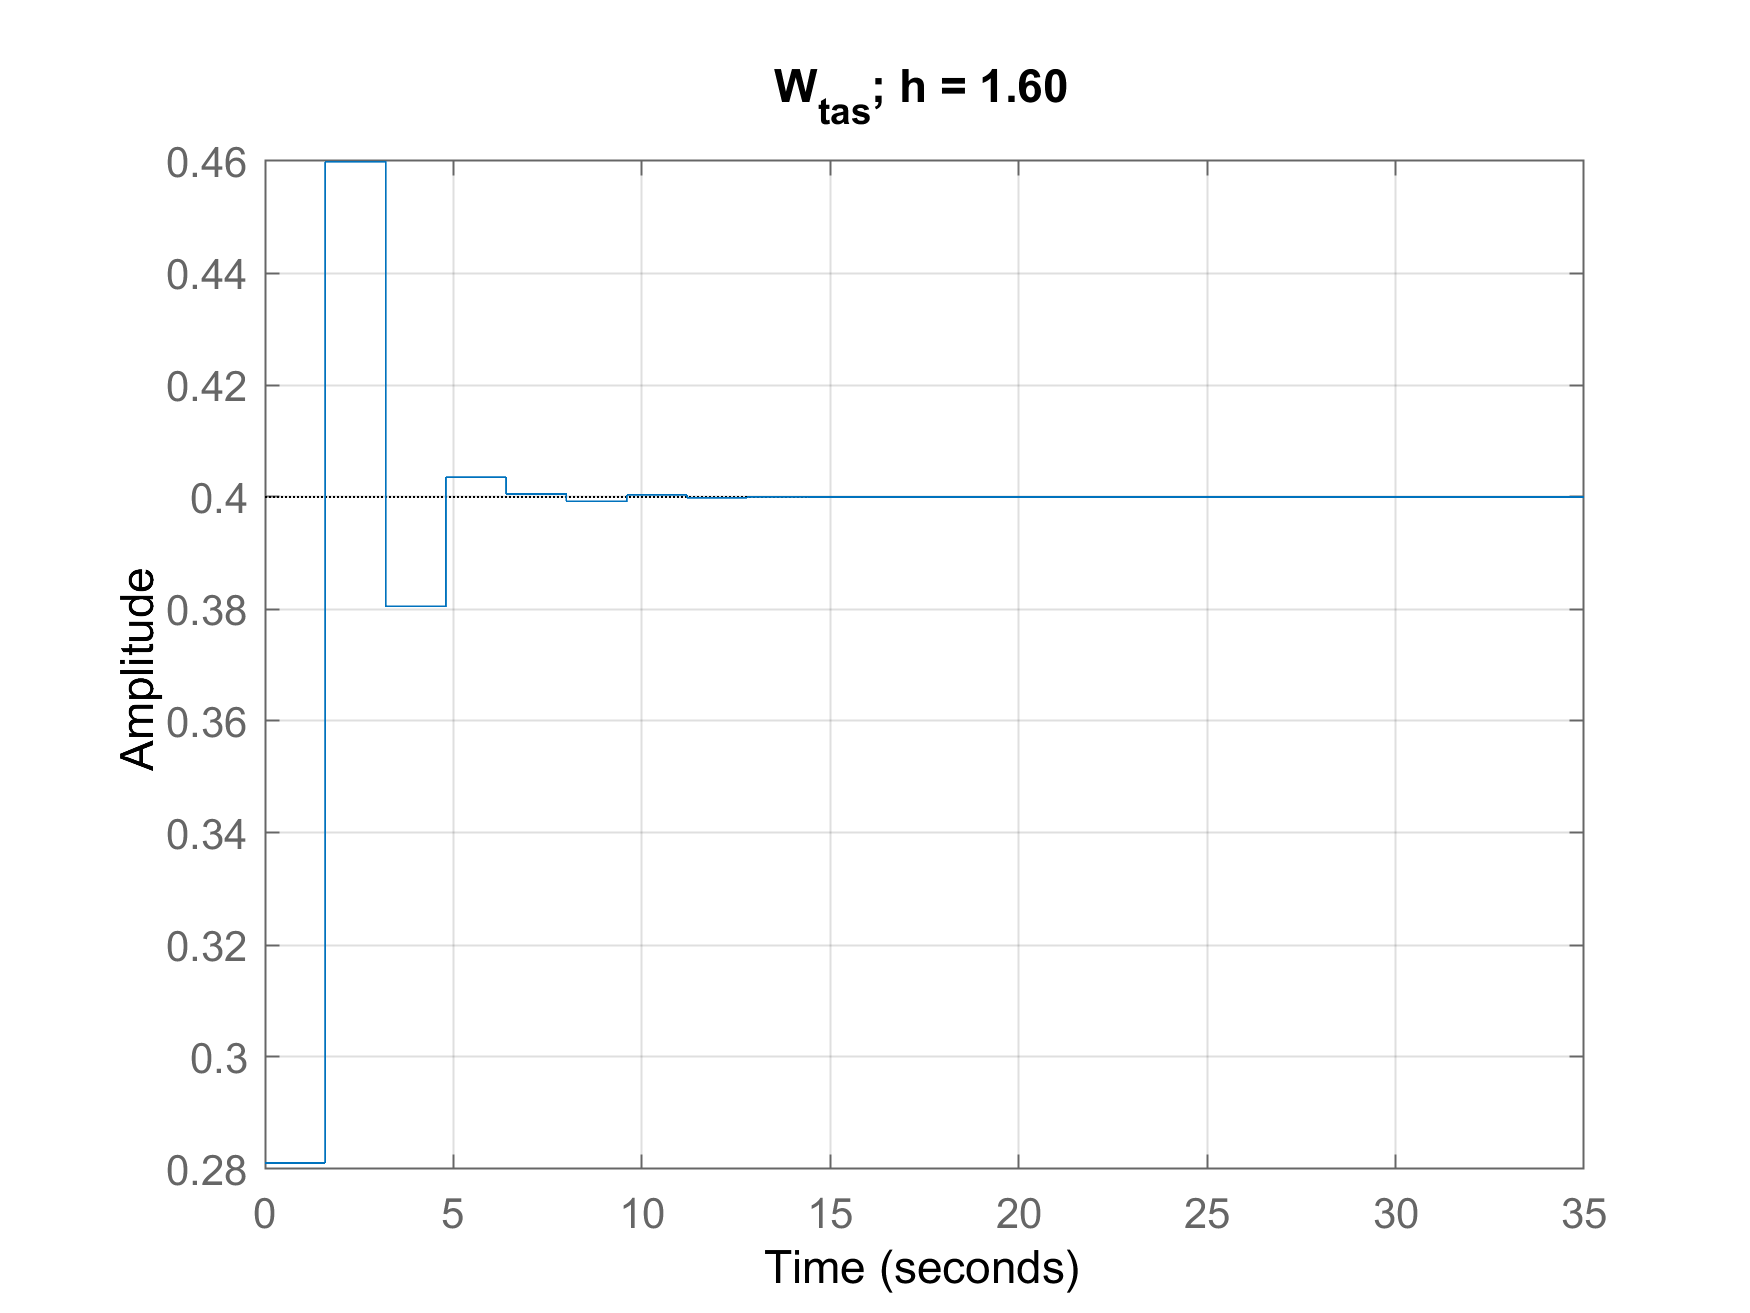
\includegraphics[width=\linewidth]{tash1.6.png}
        \end{subfigure}
        \begin{subfigure}{0.49\linewidth}
            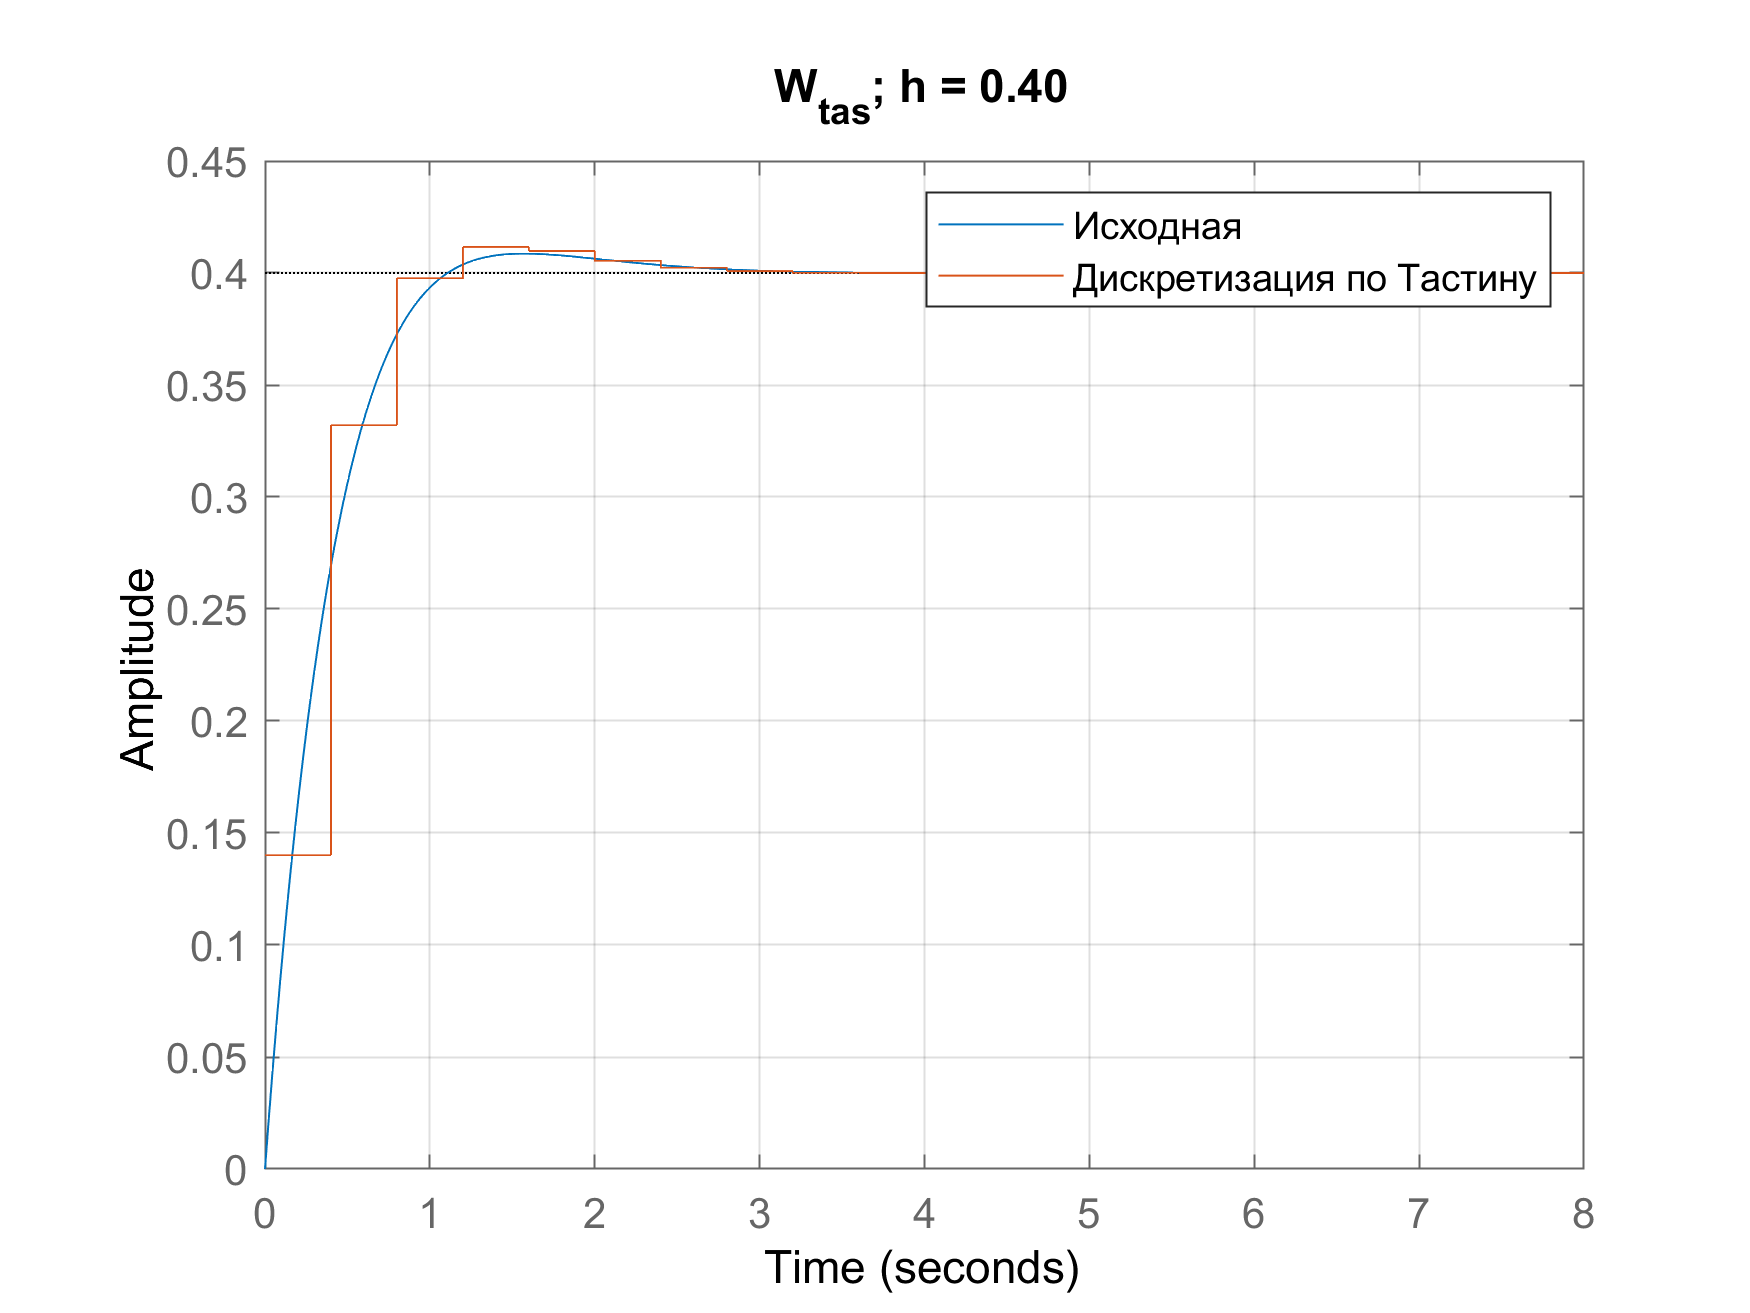
\includegraphics[width=\linewidth]{init-tash0.4.png}
        \end{subfigure}
        \caption{Переходной процесс системы дискретизированной по Эйлеру}
    \end{figure}

    \section*{Вывод}
    В лабораторной работе изучены и исследованы дискретные системы и их представления.
    В задании 3 показана эквивалентность непрерывной и дискретной систем при условии верного шага дискретизации.

    Рассмотрены методы дискретизации Эйлера и Тастина, наглядно показано влияние шага дискретизации на динамику системы.
    Также показано, что метод Эйлера при значении дискретизации больше оценочного даёт неустойчивую систему, в то время
    как метод Тастина всегда даёт устойчивую систему.

    Однако для каждой дискретной системы характерны перерегулирование и более длительный переходный процесс, чем
    для непрерывной и при снижении шага дискретизации данные параметры приближаются к параметрам непрерывной системы.
    \section*{Листинг к Заданию 3}
    \inputminted[linenos, frame=single, breakanywhere]{octave}{../src/L4T3.m}

\end{document}
